\documentclass[masters]{ucbthesis}
\usepackage[backend=biber]{biblatex}
\usepackage{graphicx}
\usepackage{float}
\usepackage{amsmath}
\usepackage{algorithm}
\usepackage{algorithmicx}
\usepackage{algpseudocode}
\usepackage{hyperref}


%%%%%%%%%%%%%%%% Commands %%%%%%%%%%%%%%%%%%%
\newcommand\myfigure[3]{
\begin{figure}[H]
\centering
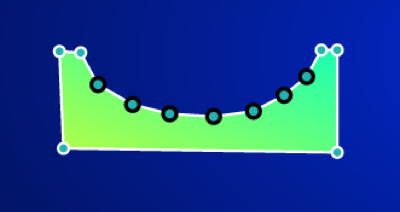
\includegraphics[#1]{figures/#2/figure.png}
\caption{#3}
\label{#2}
\end{figure}
}

\newcommand\myequation[2]{
% equation
\begin{equation}#2
	#1
\end{equation}
}

\newcommand{\specialcell}[2][c]{%
  \begin{tabular}[#1]{@{}c@{}}#2\end{tabular}}

%%%%%%%%%%%%%%%% Citations %%%%%%%%%%%%%%%%%%

\bibliography{references}

%%%%%%%%%%%%%%%%%%%%%%%%%%%%%%%%%%%%%%%%%%%%%

\begin{document}
% Declarations for Front Matter

\title{Control Sequence Generation for 2D Rotational Draining via AI Search}
\author{Peter Cottle}
\degreesemester{Fall}
\degreeyear{2012}
\degree{Masters of Science}
\chair{Professor Sara McMains}
\othermembers{Professor Tarek Zohdi}
\numberofmembers{2}
\field{Mechanical Engineering}
\campus{Berkeley, California}


\maketitle
\approvalpage
\copyrightpage

% (This is included by thesis.tex; you do not latex it by itself.)

\begin{abstract}

This paper provides several contributions related to the workpiece drainability problem in manufacturing. First we describe our parametric approach to a particle model that uses parabolic path segments rather than straight-line segments. This improvement allows for particles to maintain velocity, travel through rotating acceleration fields, and collide with workpiece edges while maintaining constant-time intersection tests per geometric primitive.

Next we provide a framework for approaching the drainability problem from an artificial intelligence perspective. We define our state space formulation and note how the size of the state space is linear with geometric features and exponential with the number of particles being drained. We then define our sampling approach to the successor function; this sampling approach allows us to discover the majority of connectivity information while only exploring a subset of the action space.

Finally, we describe how our algorithm searches for a solution to determine if a given workpiece is drainable. The primary result produced by our work is a full sequence of rotation angles throughout time to drain the workpiece; this represents a direct control sequence that can be fed into fixture rotator, providing immediate utility in industry.

%First we describe our method for
%This improvement leads to a technique for handling vertex placement
%Next, we rpovide
%Finally, we describe our method
%We survey the computational geometry relevant to, we especially focus on, we briefly survey
%We describe data structures for representing... our implementation of the data structure...

\vspace{0.2in}

\textbf{Keywords}: workpiece drainability, parametric equations, fluid simulation

\end{abstract}


\begin{frontmatter}

%\begin{dedication}
%\null\vfil
%\begin{center}
%To everyone who helped me along this journey.
%\end{center}

%\vfil\null
%\end{dedication}

\tableofcontents
\clearpage
\listoffigures
\clearpage
\listoftables

\begin{acknowledgements}
\begin{center}
To everyone who helped me along this journey.
% I would like to acknowledge Nescafe Instant Coffee, electronica music, and the burning fear of failure for motivating me to complete this work.
\end{center}
\end{acknowledgements}

\end{frontmatter}

\pagestyle{headings}

							\chapter{Introduction \& Motivation}


During the manufacturing process for engine components, many byproducts are produced that contaminate the final workpiece \cite{Hancock94}. These byproducts can include sand from sand casting, chips from additional machining, and burrs from hole-cutting \cite{Arbelaez}.
These byproducts are commonly cleaned off with high pressure water-jets; while these jets are effective at removing contaminants, they introduce large volumes of water that may settle in concave regions of the workpiece \cite{Arbelaez}. This fluid must be removed before the final stages of the manufacturing process can continue; the removal of this fluid is a non-trivial task due to complex workpiece geometry \cite{Avila} \cite{Yasui2011}. Removing this fluid from the workpiece is referred to as the ``workpiece drainability'' problem in our field.

Manufacturers and designers have two key objectives to accomplish when presented with the drainability problem. The first is to analyze the ``drainability'' of the workpiece about a given axis. Drainability is defined as the ability for the workpiece to be drained by rotation, usually in reference to a given rotation axis. Existing work has made great progress in this domain; Yasui et al.'s work is capable of producing a map of which rotation axes will fully drain the workpiece under an infinite number of rotations \cite{Yasui2011}. These results can be quite useful when designing rotation fixtures or altering the geometry of a workpiece, despite the algorithm using a simplified model of true fluid behavior.

While the drainability analysis for a workpiece is useful, it does not produce any bounds on the time required to drain the workpiece. Likewise, it also does not specify a rotation speed or total rotation angle. For this reason, manufacturers would also like to accomplish the second objective of the drainability problem -- achieving a specific sequence of rotations that fully drains the workpiece under a given rotation axis.

This sequence of rotations would be immediately useful on the manufacturing floor to input as a control sequence to a workpiece rotator. Existing work has mainly focused on analyzing drainability \cite{Yasui2011} or the number of machining operations needed to attain drainability \cite{Aloupis_draininga}. Consequently, the focus of our work presented in this paper is to produce a specific sequence of rotations for drainability. If both halves of the drainability problem can be solved, the combined solution would serve great utility in reducing time and energy required to manufacture a given part.



						\chapter{Modeling Approach}

Analyzing the drainability of a workpiece requires that the behavior of fluid throughout the workpiece be modeled in some way. This behavior is complex; trapped gases, viscuous effects, and fluid mechanics all interact during workpiece draining. There are many ways to model this fluid behavior, and each choice comes with both advantages and disadvantages.

Advanced fluid simulation methods like the finite element method or smoothed-particle hydrodynamics approximate fluid behavior with high accuracy, but their computation is quite expensive in both time and memory. This is primarily because they are integration methods -- their accuracy relies on integrating many times over a small timestep.

Thus, in order to quickly simulate fluid behavior during drainability analysis, most previous work chooses a greatly simplified fluid model. While accuracy is sacrificed by choosing a simpler model, more useful analysis can be produced by simulating many different scenarios.

\section{Straight-Line Multiple-Particle Model}

	\subsection{Core Assumptions}

Yasui et. all \cite{plot} chose a simplified particle modeling approach with a few core underlying simplifications:

\begin{itemize}
	\item Each fluid body within the workpiece is approximated as a single particle
	\item Water particles only travel in straight lines and do not maintain a kinetic state
	\item The workpiece would rotate infinitesimally slow in one direction for an infinite amount of time
\end{itemize}

	\subsection{Modeling Choice Advantages and Disadvantages}

This modeling approach allowed Yasui et. all to reduce the fluid draining problem down to a particle draining problem. Furthermore, particle simulation within the workpiece is greatly simplified; particles always travel in straight lines and do not accumulate kinetic energy. This means that all collisions are completely inelastic, and particles leaving an edge travel parallel to the acceleration field.

Consequently, particle simulation in this choice of model was essentially reduced to the intersection between lines and surfaces. Because these tests are computationally inexpensive and have a sub-linear runtime in the number of triangles within the workpiece, Yusuke et. all were able to perform many particle simulations during analysis. The end result is that for every possible rotation axis, a particle is simulated out of every concave vertex in the workpiece.

This thoroughness of simulation produces a set of results that describes the workpiece drainability of any rotation axis. This analysis serves great utility during the design stage of product creation; engineers can quickly determine if a geometry change would prevent drainability and ``seal'' off the part.

Yusuke et. all's model assumes infinitesimally slow rotation of the workpiece for an infinite amount of time. Because of the assumption about the workpiece rotation, Yusuke et. all's results produce a binary value of drainability about a particular axis rather than a direct control sequence.

If this assumption about the rotation of the workpiece could be relaxed and a  control sequence of how to drain the workpiece could be produced, manufacturers could further optimize the draining stage of product manufacturing.

This work aims to produce those complementary results while simultaneously improving the kinetic model of fluid behavior.

%	\subsection{Infinitesimally Slow Rotations}

%The assumption about workpiece rotation meant that when particles rolled out of a concave vertex, the gravity direction was always nearly perpendicular to the leading edge.

%\myfigure{width=0.5\linewidth}{prevworkgravityperp}{The gravity direction is perpendicular to concave vertex leading edges.}

%	\subsection{Inelastic Collisions}

%Since water particles do not maintain kinetic state in Yasui et all, collisions against a plane are essentially just projections onto that plane.

%\myfigure{width=0.5\linewidth}{prevworkinelasticcollision}{Demonstration of purely inelastic collisions, where velocities are projected onto the collision surface.}

\section{Parabolic Single-Particle Model}

Our work utilizes a different (but related) model of the workpiece draining problem. The results produced are complementary to Yusuke et. all's results and are ideally used in conjunction.

This model is based on the following assumptions:

\begin{itemize}
	\item The fluid in the workpiece is approximated by a single particle
	\item Water particles travel in parabolic paths that are influenced by acceleration but not aerodynamic drag
	\item The workpiece can be rotated in either direction along it's rotation axis
	\item The workpiece's rotation speed can vary in time
	\item The workpiece is a two dimensional polygonal mesh
\end{itemize}

	\subsection{Assumption Effects}

This modeling choice requires a different approach to drainability analysis than the approach used by Yusuke et all; our approach, however, draws inspiration from their previous work.

The key componenets of our approach break down into the water particle simulation (presented in Chapter 4) and the search for a drainability sequence (presented in Chapter 5).




						\chapter{Physical Simulation of Water Particles}\label{physicalChapter}

Water particle simulation is the underlying core of drainability analysis -- the behavior of the fluid (or water particles in this case) must be simulated in order to analyze when and where the fluid can leave the workpiece.

Here we present the approach to simulating straight-line water particle motion based on parametric rays (the approach used in Yasui et al.'s work) and then our modification of this approach to fit parabolic water particles.

\section{Reduced Ray Approach}

	\subsection{Underlying Kinetic Model}

Individual water particles under an acceleration field $a$ with initial position $x_0$ and initial velocity $v_0$ can be modeled with a simple kinetic equation.

\myequation{
	x(t) = x_0 + v_0 \cdot t + \frac{1}{2} a \cdot t^2
}{
	\label{eq:basickinematic}
}

Equation \eqref{eq:basickinematic} shows the basic kinematic model of a water particle.


	\subsection{Reduction to Rays}

In order to obtain particles that always travel in straight lines, one may omit the acceleration term from Equation \eqref{eq:basickinematic}. This is the approach that Yasui et al. chose to obtain straight-line particle motion \cite{Yasui2011}. Under this condition, these particles can effectively be modeled as ``rays.''

\myequation{
x(t) = x_0 + v_0 \cdot t
}{
	\label{eq:kinematicDropAccel}
}

Equation \eqref{eq:kinematicDropAccel} shows this simplified ray model. Once the motion of a particle under un-obstructed movement can be easily produced, the primary challenge of particle simulation is finding the collision points of a particle's path.

	\subsection{Parametric Equations (rays)}

There are many ways to find these intersection (or ``collision'') points. One common approach is to model the ray equation as a parametric equation \cite{glassner1989introduction} \cite{fundamentals}.

\myequation{
	\vec{x}(t) = \vec{x}_0 + \vec{v}_0 \cdot t
} {
	\label{eq:parametricRay}
}

This modeling choice is shown in Equation \eqref{eq:parametricRay} where $\vec{x}(t)$ describes the location of the particle at time $t$.

\myfigure{width=0.9\linewidth}{rayexample}{A visual depiction of a ray's component vectors and its path through time}

	\subsection{Ray Tracing}

Once particles are modeled as parametric rays, all the existing techniques and libraries from ``ray-tracing'' (a standard approach to producing 3D computer graphics) can be used to find intersection points \cite{glassner1989introduction} \cite{fundamentals}.

Ray-tracing produces 3D computer graphics by sending out rays from a camera location. If one of these rays intersects a geometric primitive in the scene, the resulting color of that ray is calculated and stored in a pixel table. These ray-primitive intersections are the fundamental computational bottleneck for ray tracing; consequently, much work has been done to optimize intersection tests. Parametric modeling of geometric primitives combined with parametric rays is the industry standard \cite{glassner1989introduction} \cite{fundamentals}.

%	\subsection{Geometric Primitive Intersections}

%Because these rays are defined parametrically, they can be substituted into the parametric definition of a geometric primitive to obtain exact solutions of intersection points. This is the primary advantage of parametric equations over integration schemes -- intersections between a ray and a geometric primitive can be solved for directly in constant time \cite{g||lassner1989introduction}.

%For example, the parametric definition of a sphere with center $C$ and radius $r$ is given in Equation \eqref{eq:sphereParametric}.

% \myequation{
% 	|\vec{X} - \vec{C}|^2 - r^2 = 0
% } {
% 	\label{eq:sphereParametric}
% }

% In Equation \eqref{eq:sphereParametric}, all points $\vec{X}$ that satisfy the equation define the surface of the sphere. In order to solve for the intersection of a ray and a sphere, the parametric equation of the ray is substituted into Equation \eqref{eq:sphereParametric} for $X$. This produces Equation \eqref{eq:sphereParametricSubbed}.

% \myequation{
% 	|(\vec{x}_0 + \vec{v}_0 \cdot t) - \vec{C}|^2 - r^2 = 0
% } {
% 	\label{eq:sphereParametricSubbed}
%}

% \myfigure{width=0.5\linewidth}{raysphere}{A demonstration of a ray intersecting with a sphere.}

% Equation \eqref{eq:sphereParametricSubbed} can be expanded algebraically to yield an equation that is quadratic in $t$. This resulting equation can then be solved using the standard quadratic formula:

% \myequation{
% 	\frac{-b \pm \sqrt{b^2 - 4ac}}{2a} = t
% } {
% 	\label{eq:quadratic}
% }

% This constant-time solution for the intersection between a parametric equation and geometric primitive will be crucial for later parts of this paper.

\section{Kinetic Parametric Approach}

While this straight-line particle approach is convenient, our model aims to examine particles with more realistic kinetic properties and paths. Consequently, we choose to not omit the acceleration term from the kinetic model of a particle. This means we combine a parametric approach with Equation \eqref{eq:basickinematic} to produce Equation \eqref{eq:freeFall} -- a parabola defined parametrically.

\myequation{
	\vec{x}(t) = \vec{x}_0 + \vec{v}_0 \cdot t + \frac{1}{2} \vec{a} \cdot t^2
}{
	\label{eq:freeFall}
}


	\subsection{Geometric Primitive Intersections}

We would like to intersect these particle paths (represented by parabolas) with geometric primitives in the workpiece for simulation purposes. Since our algorithm takes in a set of polygons that define the workpiece, the only geometric primitive of interest is a polygon edge. We will first describe the parabola-line intersection test and then present the small amount of extra validation needed for the parabola-edge intersection test.

We begin by redefining the parabola's initial point $\vec{x}_0$ as $\vec{p}$ and initial velocity $\vec{v}_0$ as $\vec{v}$ for notation purposes:

$$
\vec{x}(t) = \vec{p} + \vec{v} \cdot t + \frac{1}{2} \vec{a} \cdot t^2.
$$

This gives us a parabola defined by three vectors:

\myfigure{width=0.85\linewidth}{parablinetest2}{The parabola redefined for notation purposes.}

This parabola needs to be intersected against an arbitrary edge with starting point $\vec{s}$, direction vector $\vec{d}$, and length $|\vec{d}|$:

\myfigure{width=0.6\linewidth}{parablinetest1}{Edge for intersection test.}

We know that any point $\alpha$ on the line defined by $\vec{d}$ and $\vec{s}$ has a cross product of 0:

\myfigure{width=0.6\linewidth}{parablinetest3}{Definition of a point on the line defined by $\vec{d}$ and $\vec{s}$.}

This can be represented algebraically as

$$
(\vec{\alpha} - \vec{s}) \times \vec{d} = 0.
$$

Knowing this, we can substitute our definition of the particle's path through time into this cross product:

$$
(\vec{x}(t) - \vec{s}) \times \vec{d} = 0.
$$

We can then be expanded algebraically into:

$$
(\vec{p} + \vec{v} \cdot t + \frac{1}{2} \vec{a} \cdot t^2 - \vec{s}) \times \vec{d} = 0.
$$

In order to obtain a non-vectorized equation, we then break each vector into orthogonal components as shown in Equation \eqref{eq:brokenUp}.

$$
\vec{s} = (s_x, s_y) \qquad \vec{d} = (d_x, d_y)
$$

\myequation{
	\vec{p} = (p_x, p_y) \qquad \vec{v} = (v_x, v_y) \qquad \vec{a} = (a_x, a_y)
}{
  \label{eq:brokenUp}
}

This gives us two versions of the above equation, where the cross product operation is replaced by simple multiplication:

$$
\left [ (p_x - s_x) + v_x  t + \frac{1}{2} a_x  t^2) \right ] \cdot  d_y = 0
$$

\vspace{0.1in}

$$
\left [ (p_y - s_y) + v_y t + \frac{1}{2} a_y t^2) \right ] \cdot d_x = 0.
$$

Subtracting the second equation from the first to perform the cross product and grouping terms by the power of $t$ gives us:


\myequation{
	(\frac{1}{2} a_x d_y - \frac{1}{2} a_y ) \cdot t^2 + (v_x d_y - v_y d_x) \cdot t +
\left [ (p_x - s_x) d_y - (p_y - s_y) d_x \right ] = 0
} {
	\label{eq:parabLineTest}
}

Equation \eqref{eq:parabLineTest} can easily solved by the quadratic equation:

$$
	\frac{-b \pm \sqrt{b^2 - 4ac}}{2a} = t.
$$

Equation \eqref{eq:abc} defines variables $a$, $b$, and $c$.

\myequation{
	a = (\frac{1}{2} a_x d_y - \frac{1}{2} a_y d_x) \qquad b = (v_x d_y - v_y d_x) \qquad c = \left [ (p_x - s_x) d_y - (p_y - s_y) d_x \right ]
}{
	\label{eq:abc}
}

Solving for $t$ will yield two values, representing points along the parabola path that intersect the line defined by $\vec{d}$ and $\vec{s}$:

\myfigure{width=0.7\linewidth}{parablinetest4}{Solution points for the parabola-line intersection test.}

This concludes the parabola-line intersection tests. For our simulation purposes, we would like to determine the first point that lies on the edge defined by $\vec{d}$ and $\vec{s}$ rather than the line. This requires a small extra validation step; first, negative values of $t$ are eliminated, for these points represent the particle traveling backwards in time. Then, the smallest value of $t$ is found that produces a point that lies in between points $\vec{s}$ and $\vec{s} + \vec{d}$. If no such value exists, this parabola does not intersect the given edge.

\section{Equation Types}

Now that we have defined a parabolic path segment in parametric form and demonstrated a geometric primitive intersection test, we would like to use this equation to simulate particle movement over time. During the course of simulation however, a particle may be traveling in a variety of conditions which require modifications to Equation \eqref{eq:freeFall}. The two primary conditions that determine the modifications necessary are:

\begin{itemize}
	\item whether the workpiece is rotating,
	\item whether the particle is traveling along a workpiece edge or through open space.
\end{itemize}

These two conditions, when combined in all possible ways, produce four scenarios of particle simulation that must be modeled. The following sections cover each scenario and detail the equation used.


\section{No Rotation}

We first examine the two scenarios where no rotation of the workpiece occurs during simulation.

		\subsection{Scenario \#1: Free Fall Equation}

When the particle is moving through open space with no workpiece rotation, we consider that particle to be in basic ``free-fall.'' The particle travels through empty space subject to a constant acceleration field. The resulting motion is a parabola, and no modification to Equation \eqref{eq:freeFall} is necessary.

\myfigure{width=0.9\linewidth}{freefallequation}{Example path traced out by the ``free-fall'' equation}

		\subsection{Scenario \#2: Sliding Equation}

During simulation, a particle may also begin to travel along an edge. This usually occurs after a particle collides with an edge multiple times in a row and obtains a velocity that is parallel to the edge. Our simulation algorithm performs this test by checking if the velocity component perpendicular to the edge becomes smaller than some pre-defined $\epsilon$ value; if this is true, the particle is now under a ``sliding'' scenario.

In this scenario, the acceleration vector is projected along the surface of the workpiece. If this projected acceleration is zero, the particle will stay in place; if not, the particle will begin to ``slide'' along this edge.

We achieve the modeling of this scenario by projecting the ``free-fall'' acceleration in Equation \eqref{eq:freeFall} along the workpiece edge, which produces a straight-line path.

Note that while the particle is now traveling along an edge, the resulting equation takes on the same form as the free-fall equation; the only difference is that the acceleration is now projected. Recall that $\vec{x}(t)$ here describes the position of the particle at time $t$.

\myequation{
	\vec{x}(t) = \vec{x}_0 + \vec{v}_{0} \cdot t + \frac{1}{2}\vec{a}_{projected} \cdot t^2
}{
	\label{eq:sliding}
}

\myfigure{width=0.9\linewidth}{slidingequation}{Demonstration of the sliding equation.}

With these two formulations, the particle's path can be simulated on both edges and in open space when the acceleration field is constant (e.g. the workpiece is not rotating). Furthermore, because both of these equations are strictly quadratic in $t$, they can be substituted into the definition of geometric primitives to perform intersect tests.

\section{Rotation}

Here we begin to examine the scenarios where the workpiece is rotating during particle simulation.

In this paper, we choose our frame of reference to be the X and Y axes that define the workpiece geometry. This means that when the workpiece rotates, our frame of reference stays fixed to the workpiece. Consequently, rotation changes the orientation of the acceleration field.

We see now how this rotating acceleration field affects the following scenarios. While we originally presented the edge travel scenario (Scenario \#2) second in the ``No Rotation'' section, we will present the edge travel scenario first in the ``Rotation'' section. This will illuminate the challenges we face when simulating the last scenario presented.

		\subsection{Scenario \#3: Concurrent Rotation \& Sliding Equation}

In this scenario, the particle is traveling along a workpiece edge and the workpiece is rotating.

We know that the acceleration vector is projected along the edge during edge travel. This means that the direction of the acceleration in this scenario is fixed; only the magnitude of the projected acceleration varies as the workpiece rotates. Consequently, rotation of the acceleration field only results in the magnitude of the projected acceleration changing.

This leads to a special case of particle motion which we will refer to as ``concurrent rotation and sliding.'' We first define $\hat{a}_{projected}$ as a constant unit-vector in the direction of the edge and $|a_{projected}|(t)$ as the magnitude of the projected acceleration over time. With these two new variables, we can show the resulting formulation of this scenario in Equation \eqref{eq:slidingRotating}.

\myequation{
	\vec{x}(t) = \vec{x}_0 + \vec{v}_{0} \cdot t + \frac{1}{2}\hat{a}_{projected}  \cdot t^2 \cdot |a_{projected}|(t)
} {
	\label{eq:slidingRotating}
}

This scenario is further illustrated in Figure \ref{scenario4}.

\myfigure{width=0.6\linewidth}{scenario4}{Illustration of Scenario \#4 -- concurrent rotation and free-fall.}

If rotation occurs at a constant rate and the acceleration vector begins perpendicular to the edge, the magnitude term can be modeled as

$$
mag_{accel} = cos(\omega \cdot t)
$$

where $\omega$ is the angular velocity.

%		\subsubsection{Concurrent Rotation \& Sliding Equation Intersection}

In Equation \eqref{eq:slidingRotating}, we no longer have a formulation of particle motion that is strictly quadratic in $t$. The trigonometric terms introduced by the rotation of the workpiece make it impossible to solve for path-primitive intersections in constant time. We can, however, easily substitute in values of $t$ to determine the position of the particle at a given time.

Despite the inability to intersect these trajectories with geometric primitives in constant time, we still simulate this scenario in practice. The reason for this will be detailed after Scenario \#4 is presented, when a holistic comparison of these two scenarios can be conducted.

		\subsection{Scenario \#4: Concurrent Rotation \& Free-Fall Equation}

The fourth scenario is when the particle is traveling through open space and the workpiece is rotating. In this case, the acceleration vector is no longer projected along an edge as shown in Equation \eqref{eq:slidingRotating}. The acceleration vector now has a direction that changes in time (with a fixed magnitude), as shown in Equation \eqref{eq:freefallRotating}.

\myequation{
	\vec{x}(t) = \vec{x}_0 + \vec{v}_{0} \cdot t + \frac{1}{2}\vec{a}(t)  \cdot t^2
} {
	\label{eq:freefallRotating}
}

Here, the $\vec{a}(t)$ term describes the acceleration vector over time as the workpiece rotates. Assuming a constant rotation, this term breaks down to:

$$
a_x = cos(\alpha t) \cdot |a_g|;
$$

$$
a_y = sin(\alpha t) \cdot |a_g|.
$$

This scenario produces paths that mathematically are not parabolic, as illustrated below in Figure \ref{norotationfreefall}.

\myfigure{width=0.9\linewidth}{norotationfreefall}{Demonstration of the particle path during concurrent rotating and free-fall}

		\subsubsection{Assumption \#1 - No concurrent Rotation and Free-fall}

These non-linear trigonometric terms produce an equation that can no longer be intersected against a geometric primitive in constant-time. Intersection points can still be calculated for these path segments via approaches like Newton's method, but doing so requires additional computational time. Our approach to the draining problem requires many different particle simulations; consequently, we restrict our simulation scenarios to having constant-time intersection tests.

This restriction effectively prevents our ability to simulate particles in this ``concurrent rotation and free-fall'' scenario, leading us to our induced first assumption and restriction in this paper -- particles may not travel through open space while the workpiece is rotating.

Our results chapter provides quantitative analysis of this scenario \#4 rejection and a related justification.

		\subsubsection{Resolution of Scenario \#3}

The third scenario, concurrent rotation and sliding, similarly has a kinetic path equation that cannot be easily intersected with geometric primitives. The key difference between this scenario and scenario \#4, however, is that the particle is traveling along a known edge. Since this edge length is known as well as the duration of the turn, this particle path does \emph{not} need to be intersected with other primitives in the workpiece if it remains on the edge.

Instead, the position of the particle after the specified turn is calculated. If the particle is still on the same edge at the end of the turn, we can then proceed with simulation because we are guaranteed that the particle did not collide with any other surface during the turn. If the particle is beyond the length of the edge at the end of the turn, we do not have this no-collision guarantee and cannot proceed with simulation.

Thus although we have two scenarios where particle path and solid intersection tests are difficult, only one of them (concurrent rotation and free-fall) cannot be simulated at all. The other (concurrent rotation and sliding) can be simulated whenever the particle has not traveled beyond the edge at the end of the turn, which was the most common result during our tests.

	\section{Collisions}

Collisions occur when the path for a given particle intersects a surface inside the workpiece.

\myfigure{width=0.4\linewidth}{planarcollision}{A particle colliding with a surface and the resulting elastic collision}

After a collision occurs, the particle ``transitions'' into one of three states:

\begin{itemize}
\item The particle has come to rest and simulation terminates
\item The particle begins a new path through open space
\item The particle begins a new path along the surface of a polygon
\end{itemize}

There are many types of collisions depending on the direction of the acceleration vector, the kinetic energy that the particle contains, and the angle between surfaces on a polygon. We present the two primary collisions (or transitions) of concern:

		\subsubsection{Planar To Sliding Transition}

When a particle collides with an edge and obtains a resulting perpendicular velocity ($v_{perp}$) less than some epsilon ($\epsilon$) value, the particle transitions from free-fall to sliding along an edge.


\myfigure{width=0.5\linewidth}{planartoslidingtransition}{Particle path transition from free-fall to sliding.}


		\subsubsection{Sliding To Free-Fall Transition}

When a particle reaches the end of an edge (effectively intersecting the adjacent edge), it may enter free-fall, where it is further simulated.

\myfigure{width=0.5\linewidth}{slidingtofreefalltransition}{Particle path transition from sliding to free-fall.}

%		\subsubsection{Sliding to Planar Transition}

%		When sliding along an edge, the particle may encounter another edge. If this edge has a dot product greater than zero, it collides with the edge and enters freefall again.

%\myfigure{width=0.5\linewidth}{slidingedgecollision}{Sliding particle collision with adjacent edge at obtuse.}

%		\subsubsection{Sliding-Corner Collision}

%		If the next edge has a dot product less than or equal to 0, the particle is effectively ``trapped'' as long as the gravity vector points within the edge.

%\myfigure{width=0.5\linewidth}{slidingcornercollision}{Sliding particle collision with adjacent edge at acute angle.}

	\subsection{Conservation of Momentum}

		The only source of energy in this demo is the potential energy from gravity. Note that as the workpiece rotates, the gravity vector (and corresponding field) rotates. This means that a particle in a low-energy configuration can transition to a high-energy configuration through rotation; consequently, rotation may add energy into the system.

		\subsubsection{Settling Guarantee}

		The only addition of energy is from rotation, so in the absence of rotation, no energy is added to the system. Because the elasticity  $\kappa$ of the particle-edge collisions is chosen to be less than 1 in simulation, energy dissipates as a particle collides with other surfaces.

		This leads us to the settling guarantee: the simulation of a particle during a time period with no rotation is guaranteed to terminate in one of two ways:

\begin{itemize}
\item the particle settles into a concave vertex with a kinetic energy less than $\epsilon$, or
\item the particle exits the workpiece, which is the goal of the search.
\end{itemize}


								\chapter{Solution Search}

\section{General A.I. Search}

Artificial Intelligence search is a field of study and class of algorithms that discover (or ``search'' for) plans that turn a start state into a goal state in a determinstic world. A.I. search makes heavy use of simulation to compute solutions offline before enacting those solutions in the real world.

Based on our ability to rapidly simulate water particles and the deterministic nature of the workpiece draining problem, we choose A.I. search to compute a series of rotations that fully drain a workpiece.

	\subsection{Terminology}

In order to describe how A.I. search applies to the draining problem in manufacturing, some terminology must be defined first. In order to aid our definitions, we will use a simple positional search problem as an example. Imagine a robot placed on a grid with $M$ columns and $N$ rows that is attemping to reach a goal position $G_{pos}$

\myfigure{width=0.5\linewidth}{robotGrid}{A small positional search problem.}

The ``state'' is defined as a set of information that minimally represents the current progress to the goal. For this positional search problem, the minimal state representation would be the position tuple of the robot $(R_x,R_y)$, where $R_x$ is the horizontal position of the robot and $R_y$ is the vertical position of the robot. Here these variables can take on positive integer values up to $M$ and $N$ respectively.

For every state, the agent under control has a number of actions available to take. In our example, the robot would have the actions $North$, $South$, $East$, and $West$ available to execute.

When the agent under control takes an action, a new state is produced. The ``transition function'' is responsible for transforming a state action pair into a successor state. For example, if the robot above was in position $(M = 1, N = 2)$ and took the action $North$, the transition function would return the state $(M = 1, N = 3)$.

This transition function is also responsible for performing validity checks against the environment. In our positional search example, the transition function would be responsible for making sure the robot does not move off the grid or into a square occupied by another agent or wall. If an invalid state action pair is given to the transition function, the transition function returns $null$ to designate this invalid combination.

The ``successor function'' is a meta function that uses the transition function and available actions to the agent. It is responsible for generating a list of successor states from a given state. For the above problem, the successor function would return the list of adjacent squares the robot could move into and the actions that produce those states.

A ``plan'' is simply a sequence of actions. Plans are usually maintained and updated by the successor function when exploring states. This is because while reaching the goal state determines that the search algorithm has succeeded, the sequence of actions to achieve a goal state is usually the objective of the solution.

	\subsection{General Tree Search}

These definitions are enough to implement the standard tree search algorithm.

\begin{algorithm}[H]
\begin{algorithmic}[1]
\Function{TreeSearch}{$problem$}
	\State $queue \gets$ (initial state of $problem$, empty $plan$)

	\While{$queue$ not empty}
		\State $state, plan \gets$ REMOVE-FRONT($queue$)
		\If{Goal-Test($problem$,$state$)}
			\State \textbf{return} $plan$ \Comment{Success}
		\EndIf
		\State InsertAll($queue$, SuccessorFunction($state, plan$)) \Comment{Inserts a list of new states and plans into the queue}
	\EndWhile
	\State \textbf{return} $failure$ \Comment{Failure from exhausting all states on the queue}

\EndFunction

\end{algorithmic}
\end{algorithm}

	\subsection{Importance of Formulation}

The above definitions of state, actions, and successor functions are quite general. This means that there are several valid formulations (or definitions) of states for a given problem. The particular formulation chosen can have large consequences on the effectiveness of A.I. search and the algorithmic runtime.


The size of the state space is the important factor when considering different problem formulations. A state space size is defined by size of the set of the different values the state could hold.

For our example above, we define the state to be the position tuple $(R_x, R_y)$. Since $R_x$ and $R_y$ can take on postive integer values up until $M$ and $N$ respectively, the size of the set of possible state values is $MN$.

While a positional search problem with one agent does not present a large (or ``expansive'') state space, these state spaces can quickly get out of control for slightly more complex problems. For instance in the general case of $l$ agents on a board of $M$ by $N$ size, the state space is defined by the list of position tuples $(R^1_x, R^1_y), (R^2_x, R^2_y)... (R^l_x, R^l_y)$. In this case the size of the state space is all possible permutations of these variables, or $(MN)^l$.

State spaces often grow exponentially large with the addition of new variables. If the state space becomes too expansive, the effectiveness of general search algorithms can be jeopardized. This is because general A.I. search has to enumerate through (or ``process'') many different states before reaching a goal state. If there are too many states to process before reaching a goal state, the algorithm may not terminate in a reasonable amount of time.

\section{Adaption of A.I. Search}

This work focuses on a traditional application of A.I. search to a novel state space formulation for workpiece draining. Our unique state formulation reduces the size of the state space to make it manageable for general A.I algorithms.

	\subsection{Traditional Formulation}

Rotating a water particle out of a workpiece can be considered a kinematic planning problem. Traditional kinematic planning problems often have state spaces that encode the kinematic properties of the object (or agent) being planned for \cite{plot}. The most common state formulation is to encode the position, velocity, and acceleration of the agent as the state formulation.

The actions available to the agent at any time are usually actions that change the acceleration on the agent. The transition function integrates this kinematic state and acceleration change in time with a pre-defined accuracy. Consequently, many transition function calls must be made to accurately integrate the path of the agent through time.

The problem with this type of state formulation is that the state space commonly becomes far too expansive for general A.I. search algorithms. For example, in a reduced problem where there are only 1000 possible position, velocity, and acceleration vectors for the state, the state space is $1000^3$. This presents far too many possible states for search algorithms to enumerate through and may prevent the algorithm from terminating.

Because of this, general A.I. search is rarely used in kinematics problems -- other techniques like kinematical motion planning are more common \cite{plot}.

	\subsection{Our State Formulation}

Our state formulation overcomes these difficulties by drastically reducing the size of the state space. We instead offload most of the computational overhead to the successor function.

The key insight here is to observe only the concave vertices of the workpiece; this insight was first used by Yusuke et all \cite{plot} in order to reduce the scope of the rotation axis discovery problem. Here it is applied to the state space formulation for the first time in order to maintain the effectiveness of general A.I. search.

We define our state as the ``settled'' position of the particle, meaning the state is either:

\begin{enumerate}
\item The concave vertex the particle is resting in, or
\item outside of the workpiece.
\end{enumerate}

By defining our state this way, we produce a state space with size of
$$
num(V_{cc}) + 1
$$
where $V_{cc}$ is defined as the set of concave vertices in the workpiece. The size of this state space is small compared to kinetic state definitions which can be exponential in the accuracy of each value.

Because the maximum number of states visited is now only linear in concave vertices, our search algorithms have far fewer states to expand and a lower upper bound on running time.

\section{Exploration}

The bulk of the computational work will now be in the successor function, which is responsible for producing the set of states that are one ``action'' away from a given input state. If a given state $S_i$ is one action away from an input state $S_j$, we define $S_i$ to be ``reachable'' from $S_j$.

	\subsection{Successor Function}

The successor function produces the list of reachable states from a given input state. For our problem, this means that the successor function will produce the set of concave vertices (or workpiece exit status) reachable from a given arbitrary concave vertex.

$$
successor(V_{cc}^{i}) = \left \{ V_{cc}^{1}, V_{cc}^{2}, ...  \right \}
$$

	\subsection{Action Definition}

The ``actions'' available to our agent will be represented by the possible set of rotations of the workpiece. In this problem we choose our frame of reference to be the workpiece geometry, so the rotation of the workpiece is observed as a rotation of the gravity vector through time.

Thus, one specific action, or ``turn,'' is defined by a sweep in the gravity vector from $g_{start}$ to $g_{end}$ over a time $t_{turn}$. The interpolation function between $g_{start}$ and $g_{end}$ could take on any form, but we restrict ourselves to linear interpolation for simplicity.

	\subsection{Transition Function}

Now we have fully defined both elements for the transition function; the states are concave vertices and the actions available to the agent are specific turns.

Consequently, the transition function is then defined as a function that takes in a concave vertex and a turn; it produces the settled state of the particle after simulation.

$$
trans(V_{cc}^{i}, turn_{l}) = V_{cc}^j \qquad or \qquad exit
$$

	\subsection{Possible set of Turns}

A turn is defined by three different variables: $g_{start}$, $g_{end}$, and $t_{turn}$. These variables could take on many values, which means many different turns could be produced. Consequently, a large number of actions are available to the agent at any given state, which leads to computational explosion (yet again).


In this work, we restrict the possible set of ``turns'' from a given concave vertex to reasonable limits. The main way this is accomplished is by reducing the set of gravity vectors available and fixing the duration of the turn. By doing so, we reduce the space of all possible actions to something manageable which still represents the full range of kinetic possibilities.


To understand how the set of gravity vectors is reduced, some terminology must first be defined. A given concave vertex has two leading edges $E_1$ and $E_2$ defined by outward vectors $\vec{e}_1$ and $\vec{e}_2$.

\myfigure{width=0.5\linewidth}{edgeDefinition}{A concave vertex $V_{cc}^1$ and its two corresponding outward edge vectors $\vec{e}_1$) and $\vec{e}_2$}

We start with a full sphere of possibilities to sample $g_{start}$ and $g_{end}$ from, as shown below:

\myfigure{width=0.8\linewidth}{restriction1}{The initial set of possible vectors to sample $g_{start}$ and $g_{end}$ from.}

We first restrict the possible values of $g_{start}$. We would like $g_{start}$ to be a vector that does not induce motion of the particle; this ensures a turn that ends in $g_{start}$ does not require simulation once the turn ends. Simultaneously, we would also like any defined turn to spend the maximum amount of time inducing motion of the particle.

This means that $g_{start}$ is a vector that does not produce motion of the particle but is as close as possible to producing motion. There are only two vectors that satisfy these conditions -- the perpendicular vectors to $\vec{e}_1$ and $\vec{e}_2$.

\myfigure{width=0.8\linewidth}{restriction2}{$g_{start}$ is reduced to one of the two perpendicular vectors}

Our second restriction is that $g_{end}$ must be a vector that produces motion of the particle while simultaenously keeping the particle on the leading edge of the concave vertex. This produces two quarter-circle segements of possibilities for $g_{end}$, each of which are defined by a leading edge and the perpendicular vector to that edge.


\myfigure{width=0.8\linewidth}{restriction3}{$g_{end}$ is reduced to vectors that produce motion while keeping the particle on the leading edge}

This leaves two arcs of gravity vectors from which $g_{end}$ can be sampled.

	\subsection{Ideal Successor Function}

The ideal successor function produces the maximum set of ``reachable'' concave vertices from a given input concave vertex (and the actions to achieve those states).

Unfortunately, there are an infinite number of turns possible from each concave vertex, for $g_{end}$ can be selected from a continuous range of vectors. Clearly enumerating through every possible turn at every concave vertex is not possible.

	\subsection{Sampling}

To overcome this difficulty, we will instead sample from the continuous range of $g_{end}$ vectors and produce a limited number of turns. Each sample from this $g_{end}$ space produces a turn, which can be simulated with our transition function to produce a settled state.

Sampling from this space produces a list of defined turns (or actions). Our successor function will then examine these actions in conjunction with an input concave vertex and produce the set of reachable concave vertices.

Ideally this set of concave vertices would be identical to the set achieved by the full enumeration of the sampling space. This is not likely to happen in practice, but with careful design we can discover the majority of this set.

	\subsection{Representative Coverage Between Limits}

The way we produce the majority of this set is to obtain a representative coverage over the possible kinetic paths out of a concave vertex. This is done by choosing a sampling method that produces the most diverse set of kinetic paths.

If the possible range of $g_{end}$ vectors is defined between the limits of $0$ and $1$, then an initial best-guess sampling function may be to use uniform sampling in the form of $x$. Because acceleration effects compound with time, this uniform sampling method produces many kinetic paths that are almost identical as can be seen in figure \ref{samplingUniform}.

\myfigure{width=0.5\linewidth}{samplingUniform}{The range of kinetic paths produced from 10 samples from each side at uniform sampling. Many of the sampled kinetic paths are nearly identical and thus visually appear as one.}

A far better sampling function is to use $x^3$. This function produces many samples at the low end of the range of $g_{end}$ vectors and only a few at the higher end. These low-end samples produce accelerations that are minimally different, but since acceleration effects compound with time, they produce drastically different kinetic paths as can be seen in figure \ref{samplingCubed}.

\myfigure{width=0.5\linewidth}{samplingCubed}{The range of kinetic paths produced from 10 samples at cubed sampling. Note the resulting kinetic paths evenly cover the space after the leading edge.}

With this sampling function, we can obtain better coverage with lower computational cost.

	\section{Complete Formulation}

Now we have all the pieces to implement A.I. search. Our state is defined as the concave vertex the particle rests in (or workpiece exit). Our successor function samples from an available range of actions to produce a reasonable set of reachable concave vertices. Simply combining these two definitions together can produce an algorithm that discovers a sequence of actions to rotate a water particle out of a workpiece.

	\subsection{Graph Search}

To further increase computational efficiency, we implement two types of graph reduction in our search.

The first is by using the standard graph implementation of our search algorithm. This graph version of the algorithm prevents a state from being expanded twice. Because the connectivity graph within workpieces often has a lot of cycles, preventing more than one expansion at each state helps considerably in cutting down computational cost.

Note how this algorithm is similar to tree search but makes use of a closed set.

\begin{algorithm}[H]
\begin{algorithmic}[1]
\Function{UniformCostGraphSearch}{$problem,fringe$}
	\State $closed \gets$ an empty set
	\State $fringe \gets$ INSERT(MAKE-NODE(INITIAL-STATE[$problem$]),$fringe$)

	\While{$fringe$ not empty}
		\State $node \gets$ REMOVE-FRONT($fringe$)
		\If{Goal-Test($problem$,STATE[$node$])}
			\State \textbf{return} $node$ \Comment{Success}
		\EndIf
		\If{State[$node$] not in $closed$}
			\State add State[$node$] to $closed$
			\State $fringe \gets$ InsertAllByPriority(Expand($node, problem$), $fringe$)
		\EndIf
	\EndWhile
	\State \textbf{return} $failure$ \Comment{Failure from exhausting all states}

\EndFunction

\end{algorithmic}
\end{algorithm}

The second graph reduction is implemented directly in the successor function. When the successor function enumerates through the list of samples from the possible turns, it maintains a cost-sensitive closed set of concave vertices that are reachable. This set is keyed based on the ``cost'' of a transition, which in most cases is defined as the duration of the simulation.

By doing so, our successor function produces the optimal reduced set of concave vertices reachable from a given state. This graph reduction enqueues fewer plans onto the fringe, reducing the memory overhead and improving performance.

These two graph reductions excel in workpieces with finely-tesselated concave sections. Here, the connectivity graph is highly connected and contains many cycles. Without graph reductions, tree search would spend a lot of time expanding all the concave vertices over and over again.

\myfigure{width=0.5\linewidth}{hemisphereSection}{A tesselated concave section. The draining graph for a workpiece like this is highly connected and cyclic.}

\section{Cost}

The uniform cost graph search algorithm we use ensures the plan produced is optimal in cost. Our definition of cost however is very flexible and can be modified according to different manufacturing priorities.

		\subsubsection{Time}

The primary concern in manufacturing is often the processing time for a given procedure. In this case, the plans enqueued into the fringe are ordered by the total backward time to execute that plan. This ensures that when we dequeue a plan that ends in the goal, it has the lowest total time out of any plan on the fringe.

		\subsubsection{Energy}

Another popular concern in manufacturing is the energy required for a given procedure. If energy is the optimization goal, plans can be instead enqueued by the estimated total amount of energy required to execute that series of turns.


There are many ways to estimate the amount of energy required to execute a series of turns. The exact details are dependent on the fixture setup and associated motor; we present three simple models of energy estimation.

		\subsubsection{Energy - Rotation Angle}

The first estimation of energy is based on the total rotation angle. If friction in the bearings and motor are the primary energy losses for the draining process, plans can be enqueued by their total absolute angle change.

This model would be appropriate if the workpiece was well balanced in a fixture that produced high energy loss due to friction.

		\subsubsection{Energy - Workpiece Center of Gravity}

Another model for energy is based on the work the motor has to perform against gravity. If the workpiece's center of gravity is positioned far away from the center of rotation, the workpiece is unbalanced in the fixture. Turns that raise the center of gravity will produce counter-torques, will turns that lower the center of gravity will produce added acceleration.

% figure needed?

If this model is more appropriate for the fixture setup, the plans can be enqueued onto the fringe based on the integrated change in height for the center of gravity.

		\subsubsection{Energy - Acceleration And Deceleration}

Finally, if the workpiece is well balanced and friction in the rotator is low, the most appropriate model may be one based on acceleration and deceleration of the workpiece. While the total number of accelerations commonly scales with the total angle, these two properties are not necessarily the same.

In this case, plans can be enqueued based on their total acceleration change.

%shitton of equations needed here

	\subsection{Solution}
%TODO
		Defined as the sequence of gravity transitions from each concave vertex to produce a particle path that exits the workpiece.

\section{Control Sequence Generator}

Now that we have a solution, we need to generate a control sequence for the workpiece rotator.

	\subsection{Sample-defined Rotations}

These rotations are defined for us by the transition function.

	\subsection{Intermediary Rotations}

Between these samples we don't have anything. What we do is just interpolate between the last sample and the beginning of the next sample with a cubic bezier curve.

					\chapter{Results \& Future Work}

\section{Online Demo}

Our implementation of this paper is available online at the following url when accessed with a modern web browser:

\begin{centering}
\url{http://petercottle.com/liquidGraph/yc.html?demo}
\end{centering}

This implementation includes a graphical user interface that draws the sampling at each vertex and each path segment for a particle's full simulation. It also animates the solution search process and the final result; consequently, our implementation of this algorithm runs asychronously and is called inbetween graphical frame draws.

	\subsection{Run Time}

Because our implementation is run asychronously and performs a lot of (unnecessary) graphics processing during the solution search process, we provide both absolute time benchmarks and percentage breakdowns of CPU time between high-level functions.

The following CPU profile was collected during a solution search on a workpiece with 180 vertices, 55 concave vertices, and 21 polygons. The solution was obtained in 14.64 seconds on a Macbook Air with 1 1.86 GHz Intel Core 2 Duo and 2 GB of 1067 MHz DDR3 ram. This time, however, was obtained while a CPU profiler was running (in addition to other applications) and is not representative of the typical runtime for the algorithm.

The following breakdown on CPU time is provided to get a sense of the computation workload for each part. CPU Self time is defined as the time spent inside the function; CPU total time is defined as the time spent inside that function and the functions called from that location.

\begin{table}
\begin{tabular}{|c|c|c|}
\hline
CPU Self Time & CPU Total Time & Function \\ \hline
46.08\% & 46.08\% & Program (total time spent processing in Javascript) \\
20.61\% & 21.35\% & Graphical Path Generation \& Drawing \\
1.7\% & 2.8\% & Edge-Parabola Intersection \\
0.63\% & 0.64\% & Quadratic Solver \\
0.30\% & 0.30\% & Edge-Point Containment Test \\
0.07\% & 0.38\% & Particle edge slide \\
0.07\% & 0.11\% & Particle collision \\
0.05\% & 3.83\% & Gravity Turn Sampling \\
0.03\% & 48.74\% & Graph Search Step \\
\hline
\end{tabular}
\end{table}

An important note here is that only 46.08\% of execution time was spent doing computation; the rest was idle time used to smoothen animation.

	\subsection{Time Complexity}

The main time-intensive aspects of this algorithm are:

\begin{itemize}
\item The intersection between a particle path and the workpiece
\item The simulation of a particle until settling
\item The simulation of different ``turns'' at each concave vertex
\item The search expansion over the workpiece.
\end{itemize}

The intersection between a particle path and the workpiece is linear in the number of edges $O(E)$ in the workpiece because each edge is intersected against a given path.

A particle's full simulation duration is dependent on the elasticity $\kappa$ which controls the rate of energy dissipation. In the best case, a particle's simulation only has one path; in the worst case, the particle never stops moving if the elasticity of the system is 1. In practice we found that most particle simulations had a number of path segments that was proportional (linearly) to the number of edges in the polgyon. Thus the simulation step is $O(E)$, with $O(E)$ intersection tests, bringing us to $O(E^2).$

A full simulation is performed for every sampled turn at a given concave vertex. We restrict the number of samples to 20 in our implementation, so this step introduces a scalar constant $S$ defined as the number of samples taken at each concave vertex.

Finally, the graph search expansion over the workpiece is at worst linear in the total number of concave vertices $V_{cc}$. All together, the big order runtime is approximately $O(S \cdot E^2 \cdot V_{cc})$

\section{Future Work \& Discussion}

Further optimizations and improvements could be made to this work, namely to enhance the usability of the results and increase efficiency.

	\subsection{Heuristics for A* Search}

One standard improvement to uniform cost search is the addition of a consistent, admissible heuristic to convert the search into A* search. A heuristic is simply an estimation of the remaining cost from a state to the goal state. Admissibility of a heuristic requires that the heuristic never over-estimates the remaining cost, and consistency requires that the heuristic does not rapidly change values between states.

Heuristics are, by nature, very dependent on the problem they are being applied to. Many heuristics exist for positional search problems and other common search formulations; since our search formulation is rather unique, there is not as much prior work to draw from.

One initial idea for a heuristic would be to use the free-fall time from the current concave vertex to the outside of the workpiece bounding box. This essentially would be the optimistic estimation that the particle would free-fall immediately from the concave vertex at the next turn. While this heuristic would be admissible and consistent, it is also radially symmetric and does not take into account workpiece geometry. It is probable that better heuristics exist for this search formulation.

	\subsection{Bounding Box Method Adaption for Particle Simulation}

When intersecting rays with geometric primitives, most implementations using bounding-box methods to reduce the number of primitives tested against the ray. This bounding-box idea could be adapted to parabolic paths as well; determining which bounding boxes are needed still presents a fairly reasonable computational load, but great gains in efficiency could be made for dense workpieces with many edges.

\chapter{Extension to Multiple Particles}

We now present an extension of this work for draining multiple particles out of a workpiece. The initial adaption to our approach is fairly trivial, but the two heuristics we present shortly afterwards dramatically improve search performance.

\section{Initial Adaption}

Only two elements of our approach need to be modified in order to drain multiple particles out of a workpiece. The first is a modification to the state definition; the state is now a set of settled locations, one for each particle:

\myequation{
  (V_{cc}^{1}, V_{cc}^{2}, V_{cc}^{3}, ... , V_{cc}^{n})
} {
  \label{eq:multipleParticleState}
}

The second modification is to our successor function definition; the successor function now takes in a set of particle locations and produces a set of ``reachable'' states:

\myequation{
  successor((V_{cc}^{1}, V_{cc}^{2}, ... , V_{cc}^{n})^i) = \left \{ (V_{cc}^{1}, V_{cc}^{2}, ... , V_{cc}^{n})^1, (V_{cc}^{1}, V_{cc}^{2}, ... , V_{cc}^{n})^2, ...  \right \}
} {
  \label{eq:successorMultipleParticle}
}

With only these modifications alone we are now able to search for solutions that drain multiple particles out of the workpiece.

\subsection{Implementation}

These two modifications to our approach result in a fair number of changes in the implementation. One primary implementation difference is that now a given turn must be simulated across all particle locations. This simulation is usually performed by the transition function:

$$
trans(V_{cc}^{i}, turn_{l}) = V_{cc}^j \qquad or \qquad exit
$$

Earlier we had restricted our action space to only turns that produced motion of the particle and kept the particle on the leading edge of the concave vertex. This means there was only one possible outcome for a turn simulation -- motion of the particle was induced, and that motion began immediately when the turn was performed.

Now that any arbitrary turn can be simulated against an arbitrary particle, this guarantee no longer holds true. Consequently, we now have four possible simulation scenarios in the transition function:


\begin{itemize}
\item The particle is offscreen; a turn does not change this particle's state.
\item The turn results in no motion; any linear combination between $g_{start}$ and $g_{end}$ does not produce motion of the particle.
\item Motion of the particle starts immediately when the turn begins; $g_{start}$ is a vector that produces motion.
\item Motion of the particle starts midway through the turn; $g_{start}$ does not produce motion and $g_{end}$ does.
\end{itemize}

Because of these multiple simulation scenarios, the multiple-particle version of the transition function must be much more robust against arbitrary input. While not of great detail for the overall picture of the approach, this presents a rather large obstacle during implementation that should be considered.

\section{Multiple Particle Time Complexity}

Now that our state is defined as a set of concave vertex locations, the state space is unfortunately exponential in the number of particles, with a base defined as the number of concave vertices in the workpiece as seen below:

$$
(num(V_{cc}) + 1)^n
$$

This leads to a time-complexity that is now exponential in the number of concave vertices, rather than linear as in \eqref{eq:bigo}:

\myequation{
O(S \cdot E^2 \cdot V_{cc}^{n})
} {
  \label{eq:bigoTotal}
}

Although we earlier had avoided exponential state spaces and runtimes due to our search formulation, the introduction of multiple particles has yet again vastly expanded our state space. Our algorithm as presented thus far will still find solutions to these problems, but may spend a fair amount of time expanding unseen states to ensure optimality.

In order to improve running time of the algorithm, we present two search heuristics that greatly reduce the number of states expanded and obtain solutions much faster. These heuristics sacrifice the guarantee of optimality in exchange for an improvement in running time.

\section{Search Heuristics}

The one advantage of the multiple-particle formulation of the drainability problem is that it allows for more creativity and flexibility when composing search optimizations. Previously in single-particle draining, our state was simply defined as a concave vertex location. This meant that any potential heuristic had only the workpiece geometry and a position as input variables.

Now that our state is a set of settle locations, we can instead create heuristics that operate on direct properties of the state.

\subsection{Plan Ranking Heuristic}

The first optimization (and true search heuristic) we implemented was simply a ranking of the partial plans in the priority queue during uniform cost search. Rather than ranking only by cost, we also implemented the following two heuristics:

\begin{itemize}
\item Always prefer plans with a higher number of exited particles, regardless of cost.
\item The number of particles in the same location shall be combined with cost as the primary ranking key.
\end{itemize}

During our testing of the algorith, we found that ranking potential plans by

$$
cost - 10 \cdot numSame
$$

where $numSame$ is the number of particles in the same location produced the best mix between optimality of plans and speed of search.

With this plan ranking heuristic, our search algorithm prefers states that have a high number of particles out of the workpiece or a high number of particles in the same location. Plans that fit these characteristics have an additional performance benefit; exited particles do not have to be simulated in the transition function, and each concave vertex location only has to be simulated once.

This essentially reduces the time complexity of the algorithm. If $o$ is the number of particles that have exited the workpiece and $m$ is the number of particles in duplicate locations, the time complexity is then:

\myequation{
O(S \cdot E^2 \cdot V_{cc}^{n -o -m})
} {
  \label{eq:bigoTotalWithHeuristic}
}

Which is a factor of $V_{cc}^{o + m}$ smaller than \eqref{eq:bigoTotal}.

\subsection{Action Space Heuristic}

The second search optimization we present is centered around sampling from the action space. Recall that for a single particle, we defined our action space to sample from as a fixed set of $g_{start}$ vectors and a range of $g_{end}$ vectors that produce motion of the particle, as seen in Figure \ref{restriction3}.

Now with multiple particles, we have multiple sets of these defined vectors:

\myfigure{width=0.8\linewidth}{multiMinPocket}{Action Space sampling for each concave vertex.}

When sampling turns for our successor function, we may sample from any of these defined spaces. Doing so, however, presents three primary concerns.

\begin{itemize}
\item This action space is fairly large and grows linearly with the number of particles in the workpiece, further increasing our algorithm's time complexity.
\item Although the set of $g_{end}$ vectors for a particular concave vertex have been reduced to keep that particular particle on the leading edge of its concave vertex, a $g_{end}$ vector from this space may cause other particles to leave the surface of the workpiece during rotation. This results in scenario \#4 which causes the sample to be rejected.
\item A particular turn's $g_{start}$ may be well into the ``induce motion'' space of another concave vertex. If the workpiece would rotate infinitely fast to a particular orientation this would be of no concern, but our solution post-processor assumes that all turns inbetween partial plan turns do not induce motion. This means that in order to accurately simulate this turn, we must rotate $g_{start}$ back to the first vector that produces motion for any particle.
\end{itemize}

This third concern is the most troubling; if almost every turn must be modified during simulation, there is a potential for optimization of turn simulation.

Our approach was to simply find the one pair of $g_{start}$ vectors that do not induce motion of any particle. This is done by examining all the $g_{start}$ vectors for each concave vertex:

\myfigure{width=0.5\linewidth}{actionspace1}{$g_{start}$ vectors from each concave vertex.}

Combining all these vectors into one sample domain:

\myfigure{width=0.8\linewidth}{actionspace2}{All $g_{start}$ vectors from each concave vertex combined into one domain.}

And then selecting the pair of vectors that do not induce motion on any particle:

\myfigure{width=0.8\linewidth}{actionspace3}{Pair of $g_{start}$ vectors selected that do not produce motion of any particle.}

Now with a defined set of $g_{start}$ vectors, we can simply define the $g_{end}$ sample space as those vectors which keep all particles on a leading edge of the workpiece. This is simply the set of vectors that range from parallel to orthogonal from $g_{start}$:

\myfigure{width=0.8\linewidth}{actionspace4}{$g_{start}$ and $g_{end}$ vectors defined from a set of concave vertices.}

Now our action space is a function of the set of conacve vertex locations; this means that our action space is always the same size, regardless of the number of particles being simulated. Furthermore, we are guaranteed that every $g_{end}$ vector sampled does not cause

 This greatly improves performance of the algorithm and is a recommended heuristic to implement.


          \chapter{Results \& Future Work}\label{results}


\section{Online Demo}

Our implementation of this paper and a small solution demonstration is available online at the following url (Mozilla Firefox, Google Chrome, or Apple Safari recommended for full compatibility):

\vspace{0.2in}

\begin{centering}
\url{http://petercottle.com/liquidGraph/index.html?demo}
\end{centering}

\vspace{0.2in}

Another solution demonstration for a more complex part is available at this url:

\vspace{0.2in}

\begin{centering}
\url{http://petercottle.com/liquidGraph/yc.html?demo}
\end{centering}

\vspace{0.2in}


\newpage


\myfigure{width=0.85\linewidth}{demoFoundSolution}{A screen capture from our implementation, available online.}


This implementation includes a visualization that draws the sampling at each vertex and each particle's full path. It includes a graphical user interface for inputting and editing workpiece geometry. Lastly, it also animates the solution search process and the final result; consequently, our implementation of this algorithm runs asynchronously and is called in-between graphical frame draws.

  \subsection{Run Time}

Because our implementation is run asynchronously and performs a lot of graphics processing during the solution search process solely for visualization, we provide both absolute time benchmarks and percentage breakdowns of CPU time between high-level functions.

The following CPU profile was collected during a solution search on a workpiece with 180 total vertices, 55 concave vertices, and 21 polygons. The solution was obtained in 14.64 seconds on a Macbook Air with a 1.86 GHz Intel Core 2 Duo and 2 GB of 1067 MHz DDR3 ram. This time, however, was obtained while a CPU profiler was running (in addition to other applications) and is not representative of the typical runtime for the algorithm.

In fact, search for the solution is rate-limited by the animation engine which runs at 60 frames per second. Consequently, all computers that are capable of completing the necessary operations between frame draws will find the solution in the same amount of time, another reason why absolute computation time is not representative of performance for our work.

The following breakdown on CPU time is provided to get a sense of the computation workload for each high-level function. CPU Self time is defined as the time spent inside the function; CPU total time is defined as the time spent inside that function and the functions called from that location.

\begin{table}[H]
\centering
\label{resultsTable}
\begin{tabular}{|c|c|c|}
\hline
CPU Self Time & CPU Total Time & Function \\ \hline
46.08\% & 46.08\% & Program (total time spent processing in Javascript) \\
20.61\% & 21.35\% & Graphical path generation \& painting \\
1.7\% & 2.8\% & Edge-Parabola intersection \\
0.63\% & 0.64\% & Quadratic equation solver \\
0.30\% & 0.30\% & Edge-Point containment test \\
0.07\% & 0.38\% & Particle sliding equation \\
0.07\% & 0.11\% & Particle collision \\
0.05\% & 3.83\% & Gravity turn sampling \\
0.03\% & 48.74\% & Graph search step \\
\hline
\end{tabular}
\caption{CPU Time breakdown for a solution search}
\end{table}

An important note here is that only 46.08\% of execution time was spent doing computation; the rest was idle time used for animation.

  \subsection{Ranking Heuristic Performance Improvement}

Our plan ranking heuristic presented in Chapter \ref{multipleExtension} produced great performance improvements during multiple-particle search. Here we present a table summarizing the running time difference between a our implementation with and without this plan heuristic.

\begin{table}[H]\label{rankingHeuristicResults}
\centering
\begin{tabular}{|c|c|c|c|c|}
\hline
Test Piece URL & Number of Particles & Time without Ranking Heuristic & Time with Ranking Heuristc & Factor Improvement \\ \hline
$/index.html?demo$ & 4 & 20.672s & 7.009s & 2.949 \\ \hline
$/yc.html?demo$ & 2 & 100.947s & 62.104s & 1.625 \\ \hline
\end{tabular}
\end{table}

  \subsection{Constants}

Our implementation uses the following values for simulation constants:

\begin{table}[H]\label{constantsTable}
\centering
\begin{tabular}{|c|c|c|}
\hline
Constant Description & Symbol & Value \\ \hline
Particle Elasticity & $\kappa$ & 0.5 \\
Perpendicular Edge Velocity & $\epsilon$ & 0.9\\ \hline
\end{tabular}
\end{table}


  \subsection{Scenario \#4 Rejection}

Our preliminary tests indicate that our restriction on scenario \#4 during simulation does not have a large effect on obtaining a solution. While we are not able to determine if workpieces exist in which every solution contains a scenario \#4 particle path, we present a summary of the number of samples rejected due to this restriction below in Table \ref{scenario4rejects}.

\begin{table}[H]\label{scenario4rejects}
\centering
\begin{tabular}{|c|c|c|c|}
\hline
Test Piece URL & Total Samples & Scenario \#4 Samples Rejected & Percentage \\ \hline
$/index.html?demo$ & 3400 & 854 & 25.12\%\\
$/yc.html?demo$ & 1200 & 264 & 22\% \\ \hline
\end{tabular}
\end{table}

It is also important to note that manufacturers may prioritize obtaining \emph{any} solution to the draining problem in a reasonable amount of time over obtaining \emph{the} optimal solution (at the expense of time). If this is the case, it is reasonable to reject scenario \#4 for performance reasons.

\section{Future Work \& Discussion}

Further optimizations and improvements could be made to this work, namely to enhance the usability of the results and increase efficiency.

  \subsection{Heuristics for A* Search}

One standard improvement to uniform cost search is the addition of a consistent, admissible heuristic to convert the search into A* search. A heuristic is simply an estimation of the remaining cost from a state to the goal state. Admissibility of a heuristic requires that the heuristic never over-estimates the remaining cost, and consistency requires that the heuristic does not rapidly change values between states.

Heuristics are, by nature, very dependent on the problem they are being applied to. Many heuristics exist for positional search problems and other common search formulations; since our search formulation is rather unique, there is not as much prior work to draw from \cite{christofides1976worst}.

One initial idea for a heuristic would be to use the free-fall time from the current concave vertex to the outside of the workpiece bounding box. This essentially would be the optimistic estimation that the particle would free-fall immediately from the concave vertex at the next turn. While this heuristic would be admissible and consistent, it does not take into account workpiece geometry; consequently, the information. It is probable that better heuristics exist for this search formulation.

  \subsection{Bounding Box Method Adaption for Particle Path Intersections}

When intersecting rays with geometric primitives, most implementations using bounding-box methods to reduce the number of primitives tested against the ray. This bounding-box idea could be adapted to parabolic paths as well; determining which bounding boxes are needed still presents a fairly reasonable computational load, but great gains in efficiency could be made for complex input with many edges.

  \subsection{Adaption to 3D - Fixed Axis}

Adapting this work to 3D polygonal meshes when the rotation axis of the workpiece is fixed is mainly an exercise in implementation. The primary difference is that parabolic paths would then need to be intersected with planes in 3D space rather than edges in 2D space.

The rest of the approach, from solution search to particle simulation, would remain the same.

  \subsection{Adaption to 3D - Free Axis}

Adapting this work to 3D polygonal meshes where the workpiece can rotate about \emph{any} rotation axis at any time presents a substantially more difficult problem. The chief obstacle here is that there is an explosion of possible turns available from any given concave vertex. The final gravity vector of the turn, $g_{end}$, could be sampled from an entire sphere rather than two small arcs in a planar circle.

There may be ways to intelligently reduce the sample space and still maintain a representative coverage of the kinetic paths attainable from a concave vertex, but much work is needed before those methods can be validated.


						\chapter{Conclusion}

We have provided a new approach to the workpiece draining problem from manufacturing that produces results that are complementary to existing work.

We first described our model of the problem -- one that introduces a more accurate kinetic model of the water particles and allows for bi-directional draining with finite rotation speeds. We then introduced a parametric simulation approach that maintains constant-time intersection tests between particle paths and geometric primitives.

Finally we then combined this simulation method with a unique search formulation of the draining problem to obtain a solution. By reducing the size of the state space and offloading complexity to the transition function, we can then ``sample'' from the action space until we are satisfied with the coverage of kinetic paths.

This search formulation is then solved by standard uniform cost graph search; a solution post-processor then produces a control sequence that can be fed into machinery capable of rotating a workpiece. We believe this work makes significant progress towards a fully-realized solution for manufacturers and designers alike.


%%%%%%%%%%%%%%%%%%%%%%% Appendix and Things %%%%%
%\appendix
\printbibliography


\end{document}
